\clearpage
\section*{Memory}
The Memory Stage take \verb+iCode+, \verb+valE+, \verb+valA+, and \verb+valP+ as well as the clock signal and outputs \verb+valM+. Additionally, when writing value into memory or reading values from memory, a \verb+complete+ pulse is send when the Memory Stage is doing doing so.\\\\
Icode is fed into MemEnabler, which outputs \verb+oEnable+, \verb+wEnable+, \verb+rEnable+, \verb+addrEnable+, and \verb+datEnable+, which respectively communicate if any output is to be sent to ValM, if any value is to be written to RAM, if any value is to be read from RAM, whether the address for RAM access comes from \verb+valE+ or \verb+valA+, and whether or not the write address comes from \verb+valP+ or \verb+valA+.
\\\\
This data is written to or read from RAM using a loop to read and write data byte for byte, which is handled with a counter that starts when the pulse enters the Memory stage.  When that pulse reaches the end of memory, it signals to the next instruction that the memory stage is complete.
\subsection*{Contributors}
Arjun Kural\\
Huy Lai
\clearpage
\subsection*{Screenshots}

\begin{figure}[!ht]
    \centering
    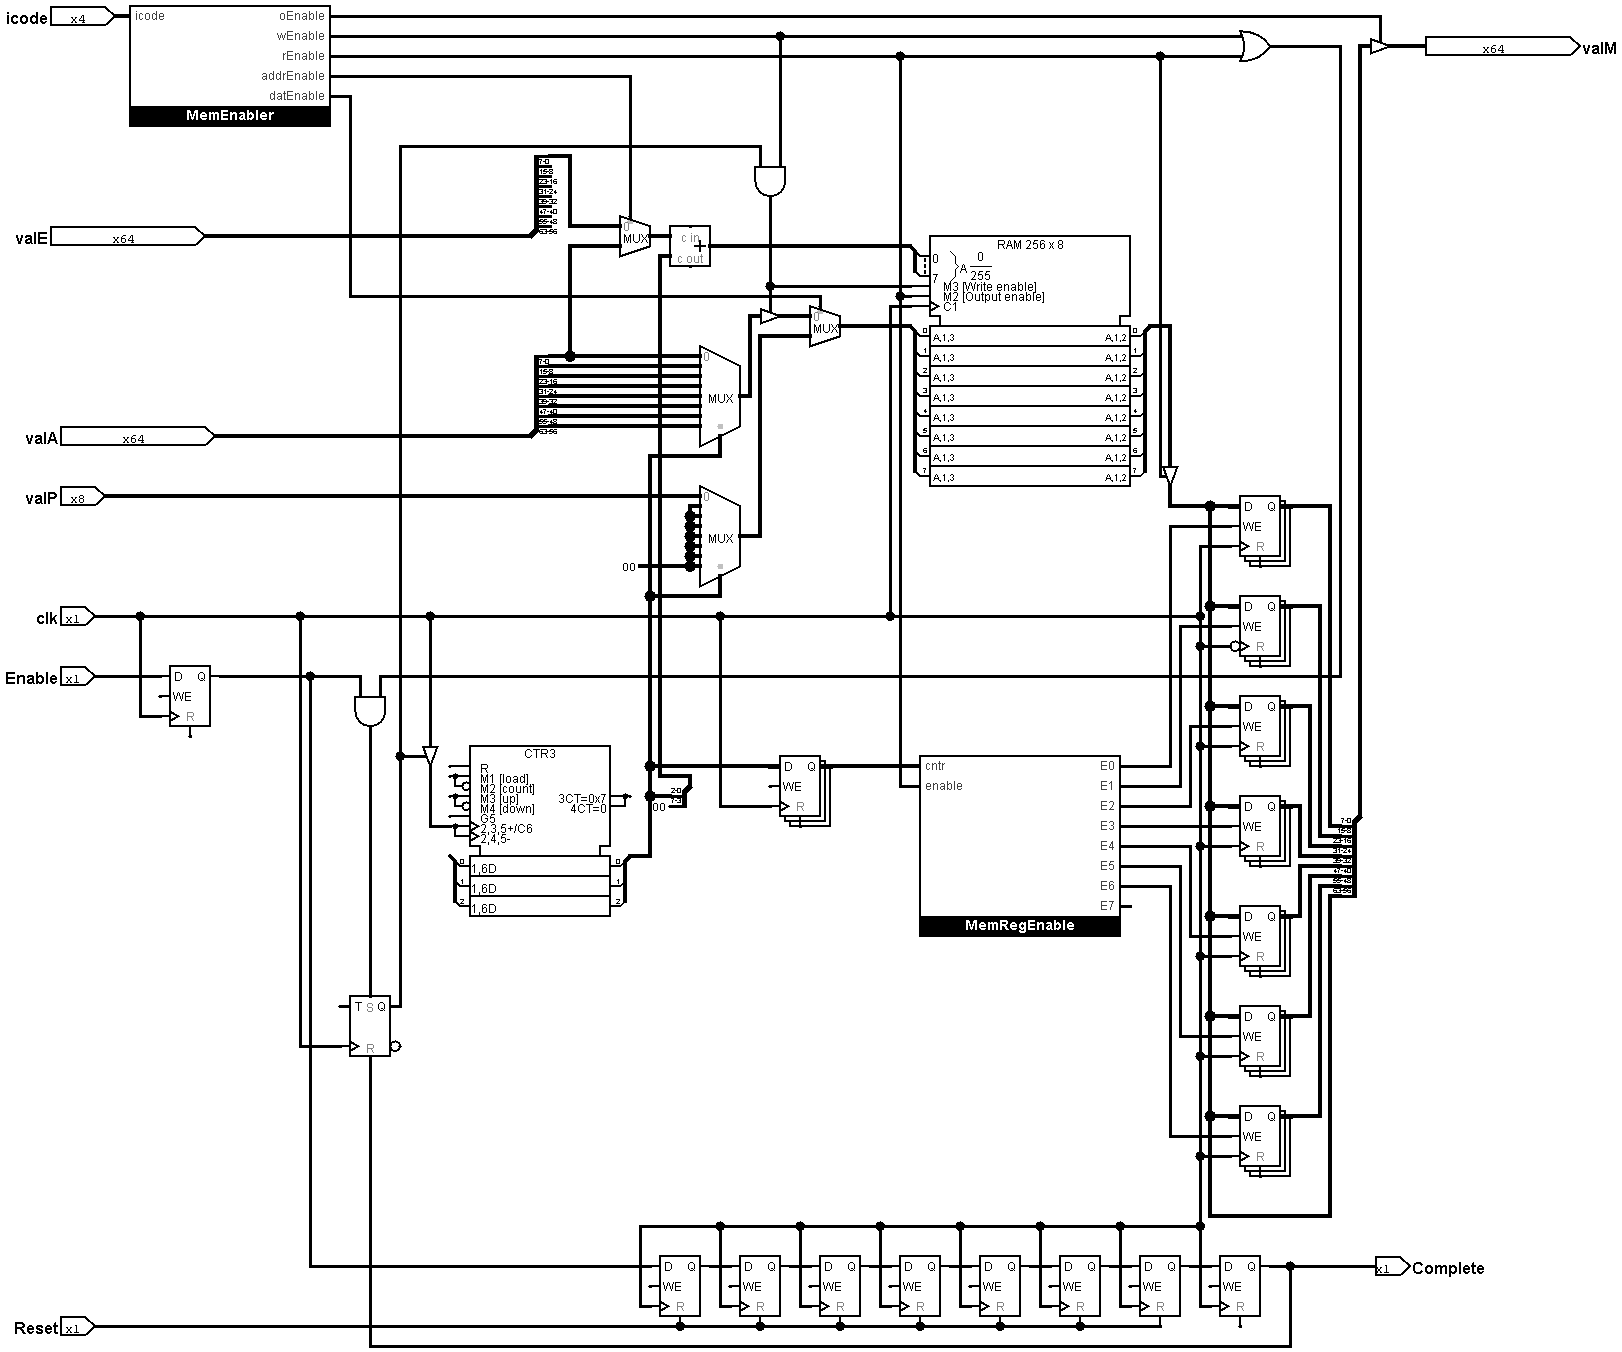
\includegraphics[width=\textwidth]{Images/Memory.png}
    \caption{Memory}
\end{figure}